%!TEX program = xelatex
\documentclass[12pt, a4paper]{article}
\usepackage[utf8]{inputenc}
\usepackage[russian]{babel}
\usepackage{pscyr}

\usepackage{xifthen}
\usepackage{parskip}
\usepackage{hyperref}
\usepackage[top=0.7in, bottom=1in, left=0.6in, right=0.6in]{geometry}
\usepackage{setspace}

\usepackage{amsmath}
\usepackage{MnSymbol}
\usepackage{amsthm}
\usepackage{mathtools}

\usepackage{algorithm}
\usepackage[noend]{algpseudocode}



\linespread{1.2}
\setlength{\parskip}{0pt}

\renewcommand\familydefault{\sfdefault}


% Stuff related to homework specific documents
\newcounter{MyTaskCounter}
\newcounter{MyTaskSectionCounter}
\newcommand{\tasksection}[1]{
	\stepcounter{MyTaskSectionCounter}
	\setcounter{MyTaskCounter}{0}
	\ifthenelse{\equal{#1}{}}{}{
	{\hfill\\[0.2in] \Large \textbf{\theMyTaskSectionCounter \enspace #1} \hfill\\[0.1in]}}
}

\newcommand{\task}[1]{
	\stepcounter{MyTaskCounter}
	\hfill\\[0.1in]
	\ifthenelse{\equal{\theMyTaskSectionCounter}{0}}{
	   \textbf{\large Задача №\theMyTaskCounter}
	}{
	   \textbf{\large Задача №\theMyTaskSectionCounter.\theMyTaskCounter}
	}
	\ifthenelse{\equal{#1}{}}{}{{\normalsize (#1)}}
	\hfill\\[0.05in]
}

% Math and algorithms

\makeatletter
\renewcommand{\ALG@name}{Алгоритм}
\renewcommand{\listalgorithmname}{Список алгроитмов}

\newenvironment{procedure}[1]
  {\renewcommand*{\ALG@name}{Процедура}
  \algorithm\renewcommand{\thealgorithm}{\thechapter.\arabic{algorithm} #1}}
  {\endalgorithm}

\makeatother

\algrenewcommand\algorithmicrequire{\textbf{Вход:}}
\algrenewcommand\algorithmicensure{\textbf{Выход:}}
\algnewcommand\True{\textbf{true}\space}
\algnewcommand\False{\textbf{false}\space}
\algnewcommand\And{\textbf{and}\space}

\newcommand{\xfor}[3]{#1 \textbf{from} #2 \textbf{to} #3}
\newcommand{\xassign}[2]{\State #1 $\leftarrow$ #2}
\newcommand{\xstate}[1]{\State #1}
\newcommand{\xreturn}[1]{\xstate{\textbf{return} #1}}

\DeclarePairedDelimiter\ceil{\lceil}{\rceil}
\DeclarePairedDelimiter\floor{\lfloor}{\rfloor}

\newcommand{\bigO}[1]{\mathcal{O}\left(#1\right)}

\makeatletter
\def\input@path{{./fig/}}
\makeatother
\graphicspath{{./fig/}}

\title{Язык запросов для геномного браузера GemlBee}
\author[Егор Горбунов]{
	\hspace{6cm} Выполнил: \hfill Егор Горбунов 
	\newline
	\hspace*{6cm} Руководитель:  \hfill Олег Шпынов
}
\institute{Кафедра математических и информационных технологий, CПбАУ}
\date{20 мая 2016 г.}

\begin{document}
\maketitle

\begin{frame}{Геномный браузер}

% \setlength{\leftmargini}{0pt}
\begin{itemize}
	\item \alert{Геномный браузер} -- приложение, отображающее различную информацию о геноме, привязанную к конкретным локациям этого генома
	\item USCS, Ensembl, BioViz, $\ldots$, \alert{GemlBee}, $\ldots$
\end{itemize}

\begin{figure}[ht!]\color{cText}\renewcommand\color[2][]{} % command to rewrite color of text in pdf_tex
\centering
\def\svgwidth{3.5in}
\input{browser.pdf_tex}
\caption{GemlBee}
\end{figure}
\end{frame}

\begin{frame}{Треки}
\begin{itemize}
	\item \alert{Трек} --- отдельная дорожка, отображаемая геномным браузером, заключающая в себе какую-то информацию про геном
	\item Бывают разные, в зависимости от этой информации
		\begin{itemize}
			\item Какая-либо статистическая информация о нуклеотидах в тех или иных частях днк
			\item Карты с конкретными генами с привязкой к участкам днк
			\item $\ldots$
		\end{itemize}
	\item Нам интересны треки, которые полезны при исследовании эпигенетических изменений (экспрессии генов)
\end{itemize}
\begin{figure}[ht!]\color{cText}\renewcommand\color[2][]{} % command to rewrite color of text in pdf_tex
\centering
\def\svgwidth{3.5in}
\input{hist.pdf_tex}
\caption{Пример трека, который нас интересует}
\end{figure}
\end{frame}

\begin{frame}{Динамическая генерация треков}
\large{\textbf{Идея:} имея результаты нескольких экспериментов, представленных в виде \emph{треков}, было бы удобно
уметь как-то комбинировать эти результаты и совершать над ними \emph{операции} с целью упрощения визуального
анализа результатов в целом.}
\end{frame}

\begin{frame}{Постановка задачи}
\large{\begin{itemize}
	\item Предложить операции, которые можно совершать над треками
	\item Сделать язык, позволяющих описывать эти операции
	\item Встроить этот язык в геномный браузер GemlBee 
\end{itemize}}
\end{frame}

\begin{frame}{Операции над треками}
\begin{itemize}
	\item Каждый трек --- это вектор из $N$ чисел
	\item Арифметические опреации ($\circ \in \{ +, -, \cdot, / \}$): $(a_1, a_2, \ldots, a_N) \circ (b_1, b_2, \ldots, b_N) = (a_1 \circ b_1, a_2 \circ b_2, \ldots, a_N \circ b_N)$
	\item Операции сравнения треков: $<$, $>$, \ldots. Результат --- \textbf{предикат} --- множество отрезков генома, на котором результат сравнения истинный
	\item Логические связки $\lor, \land, \neg$
	\item Условная генерация трека \textbf{предикату}
\end{itemize}
\end{frame}

\begin{frame}[fragile]{Язык}

\begin{lstlisting}
a := 2 + 2 

b := if (a < 1) then 1 else 3

pred := (a < b) AND (b == c)

c := (b + (if (pred) then b else a) * b) / a

show pred

show c
\end{lstlisting}

\end{frame}

\begin{frame}{Пример}
\begin{figure}
\small{
	\begin{itemize}
		\item 2 разных эксперимента по нахождению регуляторных участков днк медуллобластомы
		\item генерация треков помогает смотреть на различия результатов и пр.
	\end{itemize}
}
\centering
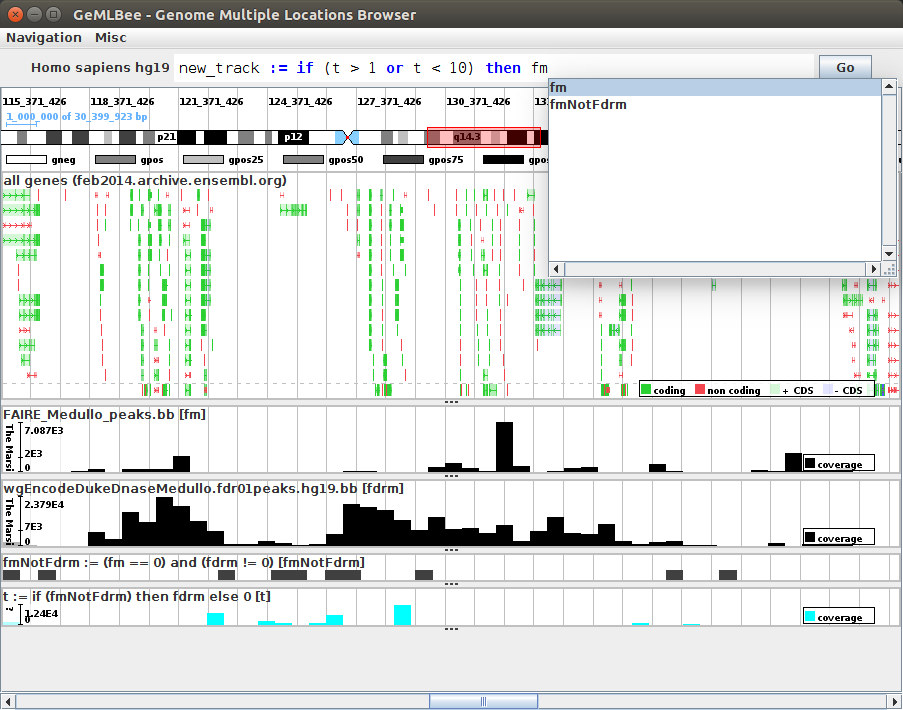
\includegraphics[width=0.7\textwidth]{ex.png}
\caption{Скриншот программы}
\end{figure}
\end{frame}

\begin{frame}{Результаты}
\alert{Что сделано:}
\begin{itemize}
	\item Реализован интерпретатор языка
	\item Язык встроен в десктопную версию GemlBee
	\item Добавлена подсветка синтаксиса и автодополнения
	\item \color{blue}{\url{https://github.com/egorbunov/gemlbee}}
\end{itemize}
\alert{Что дальше:}
\begin{itemize}
	\item Добавить поддержку в web версии GemlBee
\end{itemize}

\alert{Что узнал и что использовал:}
\begin{itemize}
	\item Kotlin
	\item Swing
	\item Parsing expression grammars
\end{itemize}
\end{frame}

\end{document}